% Diapo d'intro
\begin{frame}[c]
  \frametitle{Context}
%rajouter le titre (version courte) dans toute les slides
\begin{center}
  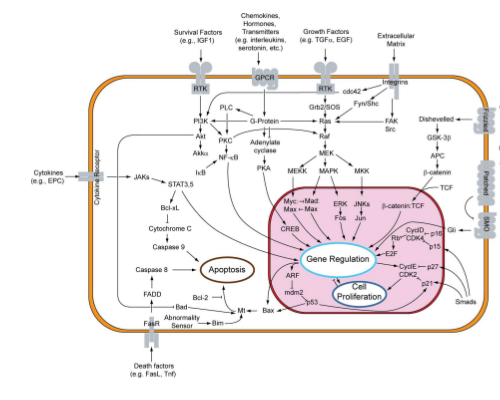
\includegraphics[scale=0.55]{images/cellule_description_lui.png}
\end{center}
\begin{center}
{\tiny \color{darkgreen}[\citelui]}
\end{center}

%\tcite{Wikipédia}

\begin{itemize}
\item Cellular processes are driven by networks of biological interactions.
\item Formal modelling and analysis of Biological Regulatory Network.
\item Static analysis of properties.
\end{itemize}

%Cellular processes are driven by networks of biological reactions. Cells rely on the tight coordination of these pathways to achieve proper functioning.
%With the help of signaling pathway, a cell senses changes in its environnement or internal state. This information is then passed on via cascades of biochemical 
%reactions to the appropriate mechanisms which respond by modifying the metabolic and transcriptiona activities. this in turn modifies the behavior of the cell.

%Consequently, the dynamics of biopathways play a crucial role in determinig cellular functions.

%Examples: circadian rhythm, the apoptosis pathway inducing programmed cell death, cell differentiation.

%\textcolor{couleurtheme}{$\Rightarrow$} \fbox{\tval{\large The need of comprehension of biological systems}} \textcolor{couleurtheme}{$\Leftarrow$}


%\textcolor{couleurtheme}{$\Rightarrow$} \fbox{\tval{\large Allow efficient translation from Process Hitting to BRN}} \textcolor{couleurtheme}{$\Leftarrow$}

\end{frame}

\begin{frame}[c]
  \frametitle{Motivation}
 \framesubtitle{stem cell differentiation}

\begin{center}
  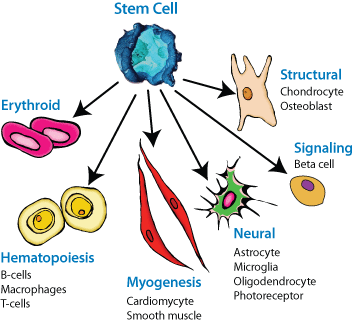
\includegraphics[scale=0.42]{images/illustration_differentiation.png}
  % \multiinclude[format=gif, scale=0.5]{images/illustration_differentiation.gif}
\end{center}
\begin{center}
{\tiny \color{darkgreen} [https://www.systembio.com/stem-cell-research/differentiation-reporters/overview]}
\end{center}
%\tcite{system Biosciences}

\begin{itemize}
\item Loss of  capability \tval{differentiation}  %expliquer la notion de perte de capacité sur la figure.
\item Which transitions (operations) are responsible of \tval{Bifurcations} ? 
\item From which state ?
\end{itemize}
\end{frame}

\begin{frame}[c]
  \frametitle{Contribution}
%system dynamique
%Bifurcations
%rajouter une autre image pour illustrer pour qu'on voit que c'est toujours des états qui changes
\begin{center}
  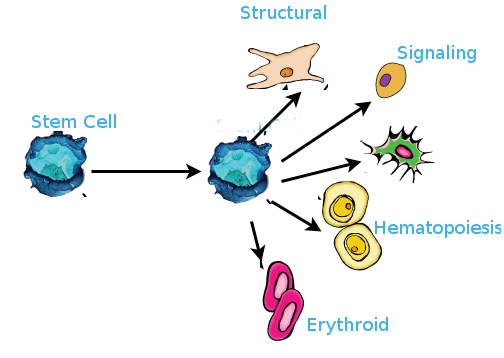
\includegraphics[scale=0.3]{images/illustration_differentiation_newio1.png}
  % \multiinclude[format=gif, scale=0.5]{images/illustration_differentiation.gif}
\end{center}


\begin{itemize}
\item Bifurcation transitions can be  expressed in temporal logic formula
\item {\bf "Relaxation"} :\\ verification of CTL formula (\tval{PSPACE (complete)})\\
       $\Rightarrow$ NP problem which can be easily expressed in SAT/ASP %trouver l'orthagraphe de easely
\item {\bf Contribution} : $$
\left\{
    \begin{array}{lcl}
        \mbox{AI (Artificial inteligence)} &\\  %rajouter un signe entre les deux
        \mbox{+} & $\Longrightarrow$ \mbox{\tval{formal approximation of bifurcations}} \\
        \mbox{AI (Abstract interpretation)} &
    \end{array}
\right.
$$ 
\end{itemize}
\end{frame}
